\documentclass[aspectratio=169,11pt]{beamer}

\usepackage{luatexja}
\usepackage{luatexja-fontspec}
\usepackage{listings}
\usepackage{tikz}
\usetikzlibrary{arrows.meta,positioning,shapes.geometric}

\setsansfont[ItalicFont={Noto Sans CJK JP}]{Noto Sans CJK JP}
\setmainjfont{Noto Sans CJK JP}
\setsansjfont{Noto Sans CJK JP}
\setmonofont{DejaVu Sans Mono}

\definecolor{Ink}{HTML}{17233C}
\definecolor{Blue}{HTML}{246BCE}
\definecolor{LightBlue}{HTML}{EAF2FD}
\definecolor{Orange}{HTML}{E87824}
\definecolor{SoftGray}{HTML}{F3F5F7}
\definecolor{CodeGray}{HTML}{4B5563}

\setbeamercolor{normal text}{fg=Ink,bg=white}
\setbeamercolor{structure}{fg=Blue}
\setbeamercolor{frametitle}{fg=Ink,bg=white}
\setbeamercolor{title}{fg=Ink}
\setbeamercolor{subtitle}{fg=Blue}
\setbeamercolor{block title}{fg=white,bg=Blue}
\setbeamercolor{block body}{fg=Ink,bg=LightBlue}
\setbeamercolor{alerted text}{fg=Orange}
\setbeamerfont{title}{size=\fontsize{25}{29},series=\bfseries}
\setbeamerfont{subtitle}{size=\large}
\setbeamerfont{frametitle}{size=\Large,series=\bfseries}
\setbeamerfont{footline}{size=\scriptsize}
\setbeamertemplate{navigation symbols}{}
\setbeamertemplate{itemize item}{\color{Blue}\raise0.2ex\hbox{\small$\blacktriangleright$}}
\setbeamertemplate{itemize subitem}{\color{Blue}\raise0.2ex\hbox{\tiny$\bullet$}}
\setbeamertemplate{blocks}[rounded][shadow=false]
\setbeamertemplate{frametitle}{%
  \vspace{0.25em}\insertframetitle\par
  \vspace{-0.3em}\color{Blue}\rule{\textwidth}{0.7pt}}
\setbeamertemplate{footline}{%
  \leavevmode\hbox{%
    \begin{beamercolorbox}[wd=.83\paperwidth,ht=2.7ex,dp=1.2ex,leftskip=.65cm]{author in head/foot}%
      \color{CodeGray}情報システム実験 I　コンパイラ演習 2026
    \end{beamercolorbox}%
    \begin{beamercolorbox}[wd=.17\paperwidth,ht=2.7ex,dp=1.2ex,rightskip=.65cm plus1fil]{date in head/foot}%
      \color{CodeGray}\hfill\insertframenumber/\inserttotalframenumber
    \end{beamercolorbox}}}

\lstdefinestyle{course}{
  basicstyle=\ttfamily\fontsize{9.2}{11.2}\selectfont,
  keywordstyle=\bfseries\color{Blue},
  commentstyle=\color{CodeGray},
  stringstyle=\color{Orange},
  showstringspaces=false,
  columns=fullflexible,
  keepspaces=true,
  frame=single,
  rulecolor=\color{LightBlue},
  backgroundcolor=\color{SoftGray},
  xleftmargin=0.5em,
  xrightmargin=0.5em,
  aboveskip=0.45em,
  belowskip=0.35em
}
\lstset{style=course}

\newcommand{\term}[1]{\textbf{\color{Blue}#1}}
\newcommand{\task}[1]{\textbf{\color{Orange}#1}}

\title{コンパイラ演習}
\subtitle{WhileLang から WebAssembly への翻訳}
\author{情報システム実験 I}
\date{2026年度 集中講義}

\begin{document}

\begin{frame}[plain]
  \vspace{1.1cm}
  {\usebeamerfont{title}\color{Ink}\inserttitle\par}
  \vspace{0.25cm}
  {\usebeamerfont{subtitle}\color{Blue}\insertsubtitle\par}
  \vspace{0.9cm}
  
\begin{tikzpicture}
    \draw[Blue,line width=2pt] (0,0) -- (5.4,0);
    \fill[Orange] (5.4,0) circle (3pt);
  \end{tikzpicture}
  \vfill
  {\small\color{CodeGray}\insertauthor\hfill\insertdate}
  \note{目安 30秒。今日はコンパイラ全体を眺めたあと、実装する部分を具体化する。}
\end{frame}

\begin{frame}{今日の到達点}
  \begin{columns}[T,onlytextwidth]
    \column{0.58\textwidth}
      \begin{itemize}\setlength\itemsep{0.7em}
        \item コンパイラが行う\term{段階的な翻訳}を説明できる
        \item 構文木を\term{仮想スタック命令}へ変換できる
        \item 命令列を\term{WebAssembly テキスト形式}へ対応づけられる
        \item テストとトレースを使って不具合の場所を絞れる
      \end{itemize}
    \column{0.36\textwidth}
      \begin{block}{18分の流れ}
        概説　4分\\[0.35em]
        翻訳例　4分\\[0.35em]
        課題とヒント　8分\\[0.35em]
        着手手順　2分
      \end{block}
  \end{columns}
  \note{目安 1分。課題のゴールはパーサ作成ではなく、後半の翻訳二段を完成させること。}
\end{frame}

\begin{frame}{コンパイラの役割}
  \centering
  \begin{tikzpicture}[node distance=1.15cm and 1.35cm,>=Latex]
    \tikzset{
      stage/.style={draw=Blue,very thick,rounded corners=2pt,fill=LightBlue,
        minimum width=3.0cm,minimum height=1.05cm,align=center,font=\bfseries},
      artifact/.style={draw=CodeGray,rounded corners=2pt,fill=SoftGray,
        minimum width=2.4cm,minimum height=0.85cm,align=center}
    }
    \node[artifact] (source) {WhileLang\\ソース};
    \node[stage,right=of source] (compiler) {コンパイラ\\意味を保って翻訳};
    \node[artifact,right=of compiler] (target) {WebAssembly\\\texttt{.wat}};
    \draw[->,line width=1.2pt,Blue] (source) -- node[above,font=\small]{入力} (compiler);
    \draw[->,line width=1.2pt,Blue] (compiler) -- node[above,font=\small]{出力} (target);
  \end{tikzpicture}
  \vspace{0.7cm}

  \begin{block}{正しさの基準}
    入力プログラムを直接実行したときと、翻訳後のプログラムを実行したときに、同じ結果が得られること。
  \end{block}
  \note{目安 1分。高速化より先に意味保存を強調する。今回は小さな言語なので対応関係が見える。}
\end{frame}

\begin{frame}{今回の翻訳パイプライン}
  \centering
  \begin{tikzpicture}[node distance=0.42cm,>=Latex]
    \tikzset{
      box/.style={draw=Blue,thick,rounded corners=2pt,fill=white,
        minimum width=2.22cm,minimum height=0.85cm,align=center},
      supplied/.style={box,fill=SoftGray},
      work/.style={box,fill=LightBlue,line width=1.4pt}
    }
    \node[box] (src) {\texttt{.while}\\ソース};
    \node[supplied,right=of src] (lex) {字句解析\\\scriptsize 配布済み};
    \node[supplied,right=of lex] (parse) {構文解析\\\scriptsize 配布済み};
    \node[work,right=of parse] (stack) {仮想命令へ翻訳\\\scriptsize 課題};
    \node[work,right=of stack] (wasm) {WATを出力\\\scriptsize 課題};
    \foreach \a/\b in {src/lex,lex/parse,parse/stack,stack/wasm}
      \draw[->,thick,Blue] (\a) -- (\b);
    \node[below=0.32cm of parse,font=\small] {構文木 AST};
    \node[below=0.32cm of stack,font=\small] {スタック命令列};
  \end{tikzpicture}
  \vspace{0.65cm}

  \begin{itemize}\setlength\itemsep{0.45em}
    \item Python は \texttt{virtual\_stack.py} と \texttt{emit\_wasm.py}
    \item C は \texttt{virtual\_stack.c} と \texttt{emit\_wasm.c}
    \item 最初に一方を選び、途中で混ぜない
  \end{itemize}
  \note{目安 1分30秒。灰色は配布済み、青は学生が実装する部分。変更範囲もここで限定する。}
\end{frame}

\begin{frame}[fragile]{式の翻訳は後置記法になる}
  \begin{columns}[T,onlytextwidth]
    \column{0.47\textwidth}
      \textbf{WhileLang}
      \begin{lstlisting}
a := a * 2;
      \end{lstlisting}
      \vspace{0.25em}
      \textbf{構文木の考え方}
      \begin{center}
      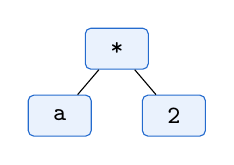
\begin{tikzpicture}[level distance=0.85cm,sibling distance=1.45cm,
        every node/.style={draw=Blue,rounded corners=2pt,fill=LightBlue,
          minimum width=0.8cm,minimum height=0.52cm,font=\small}]
        \node {\texttt{*}}
          child {node {\texttt{a}}}
          child {node {\texttt{2}}};
      \end{tikzpicture}
      \end{center}
    \column{0.49\textwidth}
      \textbf{仮想スタック命令}
      \begin{lstlisting}
rvalue a
push   2
*
lpush  a
      \end{lstlisting}
      \small
      左、右、演算子の順で並べる。演算子はスタック上の二つの値を消費し、結果を一つ積む。
  \end{columns}
  \begin{block}{実装の型}
    \texttt{compile(lhs) + compile(rhs) + [operation]}
  \end{block}
  \note{目安 2分。rvalueとlpushの違い、二項演算の順序を板書してもよい。}
\end{frame}

\begin{frame}[fragile]{WebAssembly への対応}
  \begin{columns}[T,onlytextwidth]
    \column{0.52\textwidth}
      \begin{tabular}{@{}ll@{}}
        \textbf{仮想命令} & \textbf{WAT} \\ \hline
        \texttt{push 2} & \texttt{i32.const 2} \\
        \texttt{rvalue a} & \texttt{global.get \$a} \\
        \texttt{lpush a} & \texttt{global.set \$a} \\
        \texttt{+} & \texttt{i32.add} \\
        \texttt{<} & \texttt{i32.lt\_s} \\
        \texttt{print} & \texttt{call \$print}
      \end{tabular}
      \vspace{0.65em}

      \small Wasm もスタック機械なので、多くの命令はほぼ一対一で対応する。
    \column{0.44\textwidth}
      \begin{lstlisting}
global.get $a
i32.const 2
i32.mul
global.set $a
      \end{lstlisting}
      \begin{block}{今回の範囲}
        最適化は行わない。正しい順序で命令を出すことに集中する。
      \end{block}
  \end{columns}
  \note{目安 1分30秒。i32の意味と、比較結果が1または0になる点を補足する。}
\end{frame}

\begin{frame}[fragile]{課題1 算術演算}
  \begin{columns}[T,onlytextwidth]
    \column{0.59\textwidth}
      \task{実装するもの}
      \begin{itemize}\setlength\itemsep{0.45em}
        \item 構文木 \texttt{Sub / Mul / Div} を仮想命令へ翻訳
        \item \texttt{Minus / Times} から \texttt{i32.sub / i32.mul} を出力
        \item 割り算の WAT 出力 \texttt{i32.div\_s} は配布済み
      \end{itemize}
      \vspace{0.25em}
      \begin{lstlisting}[language=Python]
case Add(lhs, rhs):
    return compile_arith(lhs) \
         + compile_arith(rhs) \
         + [Plus()]
      \end{lstlisting}
    \column{0.37\textwidth}
      \begin{block}{ヒント}
        \texttt{Add} を写し、最後の命令だけ変える。C では \texttt{bin\_arith} を使う。
      \end{block}
      \vspace{0.4em}
      \alert{順序に注意}\\
      \texttt{10 - 3} は 10、3 の順に積む。逆にすると答えが \(-7\) になる。
  \end{columns}
  \note{目安 1分30秒。Divは仮想命令側だけが課題であることを明確にする。}
\end{frame}

\begin{frame}[fragile]{課題2 比較演算}
  \begin{columns}[T,onlytextwidth]
    \column{0.48\textwidth}
      \task{実装する構文木}
      \begin{itemize}
        \item \texttt{GT}, \texttt{GE}, \texttt{LE}, \texttt{EQ}
        \item \texttt{LT} が完成例
      \end{itemize}
      \vspace{0.4em}
      \begin{lstlisting}[language=Python]
case LT(lhs, rhs):
    return compile_arith(lhs) \
         + compile_arith(rhs) \
         + [Lt()]
      \end{lstlisting}
    \column{0.48\textwidth}
      \begin{tabular}{@{}ll@{}}
        \textbf{比較} & \textbf{WAT} \\ \hline
        \texttt{>} & \texttt{i32.gt\_s} \\
        \texttt{>=} & \texttt{i32.ge\_s} \\
        \texttt{<=} & \texttt{i32.le\_s} \\
        \texttt{==} & \texttt{i32.eq}
      \end{tabular}
      \vspace{0.75em}

      真は \texttt{1}、偽は \texttt{0}。\texttt{print i > 1;} のように確認できる。
  \end{columns}
  \note{目安 1分。符号付き比較のsuffix sと、eqにはsuffixがないことを指摘する。}
\end{frame}

\begin{frame}[fragile]{課題3 while の命令列}
  \begin{columns}[T,onlytextwidth]
    \column{0.40\textwidth}
      \begin{lstlisting}
while i < 10 do
  i := i + 1;
      \end{lstlisting}
      \vspace{0.35em}
      \begin{enumerate}\setlength\itemsep{0.25em}
        \item 条件を見る場所を置く
        \item 条件が偽なら出口へ飛ぶ
        \item 本体を実行する
        \item 条件へ戻る
        \item 出口を置く
      \end{enumerate}
    \column{0.56\textwidth}
      \begin{lstlisting}
label   L.0       # test
rvalue i
push    10
<
gofalse L.1      # out
rvalue i
push    1
+
lpush   i
goto    L.0
label   L.1
      \end{lstlisting}
  \end{columns}
  \note{目安 2分。GoFalseとGoTo、testとoutの役割を一行ずつ追う。ここが講義の中心。}
\end{frame}

\begin{frame}[fragile]{while と WAT の構造}
  \begin{columns}[T,onlytextwidth]
    \column{0.53\textwidth}
      \begin{lstlisting}
(block $L.1          ;; out
  (loop $L.0         ;; test
    ... condition ...
    i32.eqz
    br_if $L.1
    ... body ...
    br $L.0
  )
)
      \end{lstlisting}
    \column{0.43\textwidth}
      \begin{block}{ラベルは二つ}
        \texttt{test}: 条件判定へ戻る先\\[0.3em]
        \texttt{out}: ループから抜ける先
      \end{block}
      \vspace{0.45em}
      \begin{itemize}\setlength\itemsep{0.45em}
        \item 入れ子ごとに \texttt{gen\_label()} で新しい名前を取る
        \item \texttt{block / loop} の出力処理は配布済み
      \end{itemize}
  \end{columns}
  \note{目安 1分30秒。Wasmのbrは任意行へのgotoではなく、構造化制御のラベルを対象にする。}
\end{frame}

\begin{frame}[fragile]{デバッグは手前から確認する}
  \begin{enumerate}\setlength\itemsep{0.48em}
    \item \term{構文木}を見る
      \quad\texttt{python3 whilec.py --ast ../test/arith.while}
    \item \term{仮想命令列}を見る
      \quad\texttt{python3 whilec.py --stack ../test/arith.while}
    \item \term{一命令ずつ実行}する
      \quad\texttt{python3 whilei.py --trace ../test/arith.while}
    \item \term{全テスト}を実行する
      \quad\texttt{python3 test\_whilelang.py}
  \end{enumerate}
  \vspace{0.45em}
  \begin{block}{切り分けの原則}
    AST が正しければパーサを疑わない。WAT の前に \texttt{whilei} を通し、仮想命令の誤りを先に直す。
  \end{block}
  \note{目安 1分30秒。Cでは./whilecと./whilei、最後はmake testに読み替える。}
\end{frame}

\begin{frame}{着手順と完了条件}
  \begin{columns}[T,onlytextwidth]
    \column{0.58\textwidth}
      \begin{enumerate}\setlength\itemsep{0.55em}
        \item Python または C を選ぶ
        \item 配布状態で \texttt{assign.while} が \texttt{3} を出すことを確認
        \item 課題1、課題2、課題3の順に実装
        \item 各段階で対応するテストを実行
      \end{enumerate}
    \column{0.38\textwidth}
      \begin{block}{主な期待値}
        \texttt{arith.while}\\
        \quad\texttt{7 8 4 23}\\[0.35em]
        \texttt{cmp.while}\\
        \quad\texttt{1 1 0 1 1 0}\\[0.35em]
        \texttt{simple\_loop.while}\\
        \quad\texttt{10}\\[0.35em]
        \texttt{fact.while}\\
        \quad\texttt{120}
      \end{block}
  \end{columns}
  \note{目安 1分。変更してよいファイルをもう一度限定し、短いテストから進める。}
\end{frame}

\begin{frame}{まとめと発展課題}
  \begin{itemize}\setlength\itemsep{0.65em}
    \item 構文木の子を順に翻訳し、最後に演算命令を置く
    \item 仮想スタック命令と WAT は多くの場合、一対一で対応する
    \item while は \texttt{test} と \texttt{out} の二つのラベルで表す
    \item 不具合は AST、命令列、実行トレースの順で切り分ける
  \end{itemize}
  \vspace{0.55em}
  \begin{block}{時間が余ったら}
    \texttt{if P then S else S} を、条件、\texttt{IfStart}、then 節、\texttt{ElseOp}、else 節、\texttt{IfEnd} の順で実装する。
  \end{block}
  \note{目安 1分。質問を受けて演習に移る。合計17分程度。}
\end{frame}

\end{document}
